\documentclass[12pt]{report}

\usepackage{lingmacros}
\usepackage{tree-dvips}
\usepackage{amsmath}
\usepackage{amsfonts}
\usepackage{hyperref}
\usepackage[english,ukrainian]{babel}
\usepackage{amsthm}
\usepackage{mathtools}

\usepackage[pdftex]{graphicx}
\usepackage{pdfpages}
\usepackage[a4paper,margin=2cm]{geometry}

\usepackage[pdftex]{graphicx}
\usepackage{pdfpages}
\usepackage[a4paper,margin=2cm]{geometry}

%% Useful packages
\usepackage{amsmath}
\usepackage{graphicx}
\usepackage{hyperref}
\usepackage{systeme}
\usepackage{titletoc}
\usepackage{array}
\usepackage{subfig}
\usepackage[font=small,labelfont=bf]{caption}
\usepackage{graphicx}
\usepackage{capt-of}

\usepackage{etoolbox}
\makeatletter
\patchcmd{\thebibliography}{%
  \chapter*{\bibname}\@mkboth{\MakeUppercase\bibname}{\MakeUppercase\bibname}}{%
  \chapter*{Література}}{}{}
\makeatother

\newtheorem{theorem}{Теорема}

\begin{document}
\begin{titlepage}
		\begin{center}
			{\largeЛЬВІВСЬКИЙ НАЦІОНАЛЬНИЙ УНІВЕРСИТЕТ ІМЕНІ ІВАНА ФРАНКА}\\
			{\Large Факультет прикладної математики та інформатики \\
			 Кафедра обчислювальної математики}
		\end{center}
	    \leavevmode \\
	    \leavevmode \\
	    \leavevmode \\
	    \leavevmode \\
		\begin{center}
			{\LARGE  Курсова робота\\}
			 на тему: \\
			\leavevmode \\
		    {\Huge \textbf{Метод інтегральних рівнянь для оберненої крайової задачі для бігармонійного рівняння}}			
		\end{center}
	    \leavevmode \\
	    \leavevmode \\
	    \leavevmode \\
	    \leavevmode \\	
	    \leavevmode \\
	    \leavevmode \\
	    \leavevmode \\
	    \leavevmode \\     
	        \begin{tabular}{p{7cm}p{12cm}}
	    	    \, & {\large Студентки IV курсу групи ПМП-41} \\
	    	    \, & {\large Напряму підготовки ``Прикладна математика''} \\
	    	    \, & {\large Багрій А. Г.} \\
	    	    \, & \, \\
	    	    \, & {\large Керівник:} \\
	    	    \, & {\large проф. Хапко Р. С.} \\
	    	    \, & {\large Національна шкала: \underline{\hspace{3cm}}} \\
	    	    \, & {\large Кількість балів: \underline{\hspace{3cm}}} \\
		    \, & {\large Оцінка ECTS: \underline{\hspace{3cm}}}
	        \end{tabular}
        \leavevmode \\
        \leavevmode \\
        \leavevmode \\
        \leavevmode \\
        \vfill
        \begin{center}
        	{\Large Львів-2020}
        \end{center}
\end{titlepage}

\tableofcontents

% 1 // Формулювання %

\chapter*{Вступ}
\addcontentsline{toc}{chapter}{Вступ}
 
 \quad Обернені задачі, які полягають у реконструкції межі області, є популярним напрямом для дослідження, оскільки такі задачі мають велику кількість застосувань. Реконструкція межі області є нелінійною задачею, що призводить до труднощів як в теоретичних дослідженнях, так і в чисельному розв'язуванні. Найбільш ефективні чисельні методи для даної задачі базуються на інтегральних рівняннях. 
 
 У даній роботі розглянуто реконструкцію внутрішньої межі двозв'язної пластини із заданими крайовими умовами, що задають певний фізичний сенс. Оскільки обернені задачі вимагають розв'язності відповідної прямої задачі, то також показано її коректність і наведено чисельні експеременти, що підтверджують теоретичні обґрунтування.

 \section*{Постановка задачі}
Нехай $\Omega\subset \mathbb{R}^2$ деяка двоз'язна область з межею $\Gamma=\Gamma_1\cup\Gamma_2$, де $\Gamma_1$ є внутрішньою межею і $\Gamma_2$ - зовнішньою. Розглянемо

\begin{equation}
	\left\{
	\label{directProblem}
	\begin{split}
		&\Delta^2 u(x)=0, \quad x\in\Omega, \\
		&u(x)=\frac{\partial u(x)}{\partial n}=0, \quad x\in\Gamma_1, \\
		&\frac{\partial u(x)}{\partial n}=g(x), \quad x\in\Gamma_2, \\
		&Mu(x)=q(x), \quad x\in\Gamma_2,
	\end{split}
	\right.
\end{equation}

\begin{equation}
	\label{dataEq}
	u(x)=f(x), \quad x\in\Gamma_2,
\end{equation}
де 
$$\Delta^{2}u(x)=\frac{\partial^{4}}{\partial x_1^4}u(x)+2\frac{\partial^{4}}{\partial x_1^2\partial x_2^2}u(x)+\frac{\partial^{4}}{\partial x_2^4}u(x) \textrm{ - бігармонійний оператор,}
$$
 $$u(x)=u(x_1,x_2) \in C^2(\Omega)\cap C(\overline{\Omega}) \textrm{ - функція, що задовольняє рівняння і крайові умови}, $$
 $$n=(n_1, n_2) \textrm{ - зовнішня нормаль до }\Gamma,$$ 
 $$Mu=\nu\Delta u+(1-\nu)(u_{x_1 x_1}n_1^2+2u_{x_1 x_2}n_1 n_2+u_{x_2 x_2}n_2^2) \textrm{ - згинальний момент пластини } \Omega,
 $$ 
 $\nu\in (0, 1)$ - коефіцієнт Пуассона і $g(x), \ q(x),\  f(x)$ - деякі задані функції, тотожньо відмінні від нуля.
 
Обернена задача \eqref{directProblem}-\eqref{dataEq} полягає у знаходженні невідомої межі $\Gamma_1$ для заданих функцій $g(x), q(x), f(x)$. Дана задача є нелінійною, оскільки її розв'язок нелінійно залежить від невідомої межі $\Gamma_1$, і також некоректною в сенсі відсутності стійкості за вхідними данними.

Перш за все, необхідно розглянути питання існування та єдиності розв'язку оберненої задачі \eqref{directProblem}-\eqref{dataEq}.

\begin{theorem}[Існування і єдиність розв'язку оберненої задачі]

Нехай $\tilde{\Gamma}_1$, $\Gamma_1$ - замкнені криві, що містяться всередині $\Gamma_2$, $\tilde{u}$, $u$ - розв'язки задачі $\eqref{directProblem}$ для $\tilde{\Gamma}_1$ і $\Gamma_1$ відповідно. Нехай $g\neq 0, q\neq 0$ i $u = \tilde{u}$ на відкритій підмножині $\Gamma_2$. Тоді $\tilde{\Gamma}_1=\Gamma_1$.

\end{theorem}

\begin{proof}

Доведемо від протилежного. Нехай $\tilde{\Gamma}_1\neq\Gamma_1$.
Нехай $\Omega_2$ - область, обмежена $\Gamma_2$, $\Omega_1$, $\tilde{\Omega}_1$ - області обмежені $\Gamma_1$, $\tilde{\Gamma}_1$ відповідно. 
\begin{equation}
W:=\Omega_2\setminus(\Omega_1\cup\tilde{\Omega}_1), \quad \Gamma_2\subset\partial W. \nonumber
\end{equation}
За теоремою Гольмгрена \cite{Holmgren} маємо $u = \tilde{u}$ в $W$. Без втрати загальності приспустимо, що $W^{*}:=(\Omega_2\setminus \overline{W})\setminus\Omega_1$ непорожня множина. Тоді $u$ є визначена в $W^{*}$ як розв'язок задачі \eqref{directProblem} для $\Gamma_1$. Вона є неперервною в $\overline{W}^{*}$ і задовольняє граничні умови на $\partial W^{*}$. Ця гранична умова випливає з того, що кожна точка з $W^{*}$ належить або $\Gamma_1$, або $\partial W\cap\tilde{\Gamma}_1$. Для $x\in\Gamma_1$ маємо $u(x)=0$ як наслідок граничних умов для $u$, для $x\in\tilde{\Gamma}_1$ маємо $u(x)=\tilde{u}(x)$ і тому $u(x)=0$ як наслідок граничних умов для $\tilde{u}$. Тоді за принципом максимуму $u=0$ в $W^{*}$ і тому $u=0$ в $D$. Це суперечить тому, що $g\neq 0, q\neq 0$.

\end{proof}


% 2 // Теореми %
\setcounter{secnumdepth}{1}
\chapter{Загальні положення}
\label{chapter1}

\section{Зведення до ІР}

Фундаментальний розв'язок бігармонійного рівняння в $\mathbb{R}^2$ має вигляд
 \begin{equation}
 	G(x, y)=\frac{1}{8\pi}|x-y|^2\ln|x-y|, \quad x,\ y \in \mathbb{R}^2.
 \end{equation}

Розглянемо потенціал простого шару для бігармонійного рівняння \cite{chapko} з густинами $\varphi$, $\psi$, що визначені на $\Gamma$:

\begin{equation}
	 	u(x)=\int_{\Gamma}\bigg(G(x,y)\varphi(y)+\frac{\partial G(x,y)}{\partial n_y}\psi(y)\bigg)d\sigma_y, \quad x\in \Omega. \nonumber
\end{equation}

\begin{theorem}[Існування і єдиність розв'язку прямої задачі]
Існує єдиний розв'язок прямої крайової задачі \eqref{directProblem}, який можна подати у вигляді
	 \begin{equation}
	 	u(x)=\sum_{k=1}^{2}\int_{\Gamma_k}\bigg(G(x,y)\varphi_k(y)+\frac{\partial G(x,y)}{\partial n_y}\psi_k(y)\bigg)d\sigma_y+\omega(x), \quad x\in \Omega,
	 \end{equation}
	 де $\omega(x) = \alpha_0+\alpha_1x_1+\alpha_2x_2 \ ((\alpha_0,\alpha_1,\alpha_2)\in R^3), \varphi_k,\psi_k\in C(\Gamma_k), k=1,2$, і невідомі густини визначаються з системи інтегральних рівнянь
	 \begin{equation}
	 \left\{
	 	\begin{split}
		\label{system}
	 		&\sum_{k=1}^{2}\int_{\Gamma_k}\bigg(G(x,y)\varphi_k(y)+\frac{\partial G(x,y)}{\partial n_y}\psi_k(y)\bigg)d\sigma_y+\omega(x)=0, \ x\in\Gamma_1, \\
			&\sum_{k=1}^{2}\int_{\Gamma_k}\bigg(\frac{\partial G(x,y)}{\partial n_x}\varphi_k(y)+\frac{\partial^2 G(x,y)}{\partial n_y\partial n_x}\psi_k(y)\bigg)d\sigma_y+\frac{\partial\omega(x)}{\partial n}=0, \ x\in\Gamma_1, \\
			&\sum_{k=1}^{2}\int_{\Gamma_k}\bigg(\frac{\partial G(x,y)}{\partial n_x}\varphi_k(y)+\frac{\partial^2 G(x,y)}{\partial n_y\partial n_x}\psi_k(y)\bigg)d\sigma_y+\frac{\partial\omega(x)}{\partial n}=g(x), \ x\in\Gamma_2, \\
			&\sum_{k=1}^{2}\int_{\Gamma_k}\bigg(M_x G(x,y)\varphi_k(y)+\frac{\partial M_x G(x,y)}{\partial n_y}\psi_k(y)\bigg)d\sigma_y+M_x\omega(x)=q(x), \ x\in\Gamma_2, \\
			&\sum_{k=1}^{2}\int_{\Gamma_k}\varphi_k(y)d\sigma_y=A_0, \\
			&\sum_{k=1}^{2}\int_{\Gamma_k}(y_1\varphi_k(y)+n_1(y)\psi_k(y))d\sigma_y=A_1, \\
			&\sum_{k=1}^{2}\int_{\Gamma_k}(y_2\varphi_k(y)+n_2(y)\psi_k(y))d\sigma_y=A_2,
		\end{split}
	\right.
	 \end{equation}
	для заданих $(A_0,A_1,A_2)\in R^3$.
 \end{theorem}
 
 Константи $A_0, A_1, A_2$ вибираються довільним чином, однак є некоректним брати за значення нулі.
 
 З умови \eqref{dataEq} маємо наступне інтегральне рівняння
 \begin{equation}
 \label{dataEq1}
	\sum_{k=1}^{2}\int_{\Gamma_k}\bigg(G(x,y)\varphi_k(y)+\frac{\partial G(x,y)}{\partial n_y}\psi_k(y)\bigg)d\sigma_y+\omega(x)=f(x), \ x\in\Gamma_2.
 \end{equation}
 

В системі \eqref{system} ядра мають вигляд
 \begin{equation*}
 	\frac{\partial G(x,y)}{\partial n_y}=-\frac{1}{8\pi}n(y)\cdot(x-y)(1+2\ln|x-y|),
 \end{equation*}
\begin{equation*}
 	\frac{\partial G(x,y)}{\partial n_x}=\frac{1}{8\pi}n(x)\cdot(x-y)(1+2\ln|x-y|),
 \end{equation*}
 \begin{gather*}
 	\frac{\partial^2 G(x,y)}{\partial n_x\partial n_y}=\frac{\partial^2 G(x,y)}{\partial n_y\partial n_x}=-\frac{1}{8\pi}\bigg(2\frac{n(x)\cdot(x-y)n(y)\cdot(x-y)}{|x-y|^2} \\
	+n(x)\cdot n(y)(1+2\ln|x-y|)\bigg),
 \end{gather*}
 \begin{gather*}
 	M_x G(x,y)=\frac{1+3\nu}{8\pi}+\frac{(1-\nu)(n(x)\cdot(x-y))^2}{4\pi|x-y|^2}+\frac{(1+\nu)\ln|x-y|^2}{8\pi},
 \end{gather*}
 \begin{gather*}
 	\frac{\partial M_x G(x,y)}{\partial n_y}=\frac{1-\nu}{2\pi}\Big(\frac{(n(x)\cdot(x-y))^2n(y)\cdot(x-y)}{|x-y|^4}-\frac{n(x)\cdot n(y)n(x)\cdot(x-y)}{|x-y|^2} \Big) \\
	-\frac{(1+\nu)n(y)\cdot(x-y)}{4\pi|x-y|^2}.
 \end{gather*}

\begin{theorem}
Обернена крайова задача \eqref{directProblem}-\eqref{dataEq} еквівалентна системі інтегральних рівнянь \eqref{system}-\eqref{dataEq1}.
\end{theorem}

 % 
\section{Алгоритм знаходення розв'язку оберненої крайової задачі}

Знаходження розв'язку задачі \eqref{system}-\eqref{dataEq1} складається з наступного ітераційного процесу:
\begin{itemize}
  \item Для заданого початкового наближення $\Gamma_1$ розв'язуємо пряму задачу для \eqref{system} і знаходимо невідомі густини.
  \item Лінеаризуємо рівняння \eqref{dataEq1} і покращуємо $\Gamma_1$, розв'язуючи лінеаризоване рівняння \eqref{dataEq1} для фіксованих густин, які є відомими з \eqref{system}.
  \item Умовою зупинки може бути $||q||_2  <\epsilon$, де $q$ - функція, що задає покращення  $\Gamma_1$, $\epsilon$ - задана точність.
\end{itemize}


% 3 // ПРЯМА ЗАДАЧА %
\chapter{Чисельне розв'язування коректної системи ІР}

% 3.1 // Параметризація %
\section{Параметризація}


Припустимо, що криві $\Gamma_1$ i $\Gamma_2$ достатньо гладкі і їх можна подати у параметричному заданні 
 
 \begin{equation}
 	\Gamma_l=\left\{x_l(s)=(x_1{_l}(s),x_2{_l}(s)) \ : \ s\in [0,2\pi]\right\},
  \end{equation}
 де $x_l \ (l=1,2)$ - аналітична, $2\pi$-періодична функція, $|x'(s)|>0.$
 Тоді систему \eqref{system} можна подати у вигляді
 
 \begin{equation}
 		\left\{
	 	\begin{split}
		\label{paramSystem}
	 		&\frac{1}{2\pi}\sum_{k=1}^{2}\int_{0}^{2\pi}\bigg(H_1{_k}(s, \sigma)\varphi_k(\sigma)+\tilde{H}_1{_k}(s, \sigma)\psi_k(\sigma)\bigg)d\sigma+\omega(x_1(s))=0,\\
			&\frac{1}{2\pi}\sum_{k=1}^{2}\int_{0}^{2\pi}\bigg(\tilde{\tilde{H}}_1{_k}(s, \sigma)\varphi_k(\sigma)+\hat{H}_1{_k}(s, \sigma)\psi_k(\sigma)\bigg)d\sigma+\frac{\partial\omega(x_1(s))}{\partial n_1}=0, \\
			&\frac{1}{2\pi}\sum_{k=1}^{2}\int_{0}^{2\pi}\bigg(\tilde{\tilde{H}}_2{_k}(s, \sigma)\varphi_k(\sigma)+\hat{H}_2{_k}(s, \sigma)\psi_k(\sigma)\bigg)d\sigma+\frac{\partial\omega(x_2(s))}{\partial n_2}=g(x_2(s)), \\
			&\frac{1}{2\pi}\sum_{k=1}^{2}\int_{0}^{2\pi}\bigg(\hat{\hat{H}}_2{_k}(s, \sigma)\varphi_k(\sigma)+\bar{H}_2{_k}(s, \sigma)\psi_k(\sigma)\bigg)d\sigma+M_x\omega(x_2(s))=q(x_2(s)),\\
			&\sum_{k=1}^{2}\int_{0}^{2\pi}\varphi_k(\sigma)d\sigma=A_0, \\
			&\sum_{k=1}^{2}\int_{0}^{2\pi}(x_1{_k}\varphi_k(\sigma)+n_1(x_k(\sigma))\psi_k(\sigma))d\sigma=A_1, \\
			&\sum_{k=1}^{2}\int_{0}^{2\pi}(x_2{_k}\varphi_k(\sigma)+n_2(x_k(\sigma))\psi_k(\sigma))d\sigma=A_2, \\
		\end{split}
		\right.
\end{equation}

Тут $ \label{kernels} \varphi_l(s) :=\varphi_k(x_l(s))|x'_l(s)|, \ \psi_l(s) :=\psi_k(x_l(s))|x'_l(s)| \ - \ \textrm{невідомі густини} $ і ядра мають вигляд
 
 \begin{equation}
 \begin{split}
	&H_l{_k}(s, \sigma) = G(x_l(s),x_k(\sigma)), \quad \tilde{H}_l{_k}(s, \sigma)=\frac{\partial G(x_l(s),x_k(\sigma))}{\partial n_y}, \\
	&\tilde{\tilde{H}}_l{_k}(s, \sigma)=\frac{\partial G(x_l(s),x_k(\sigma))}{\partial n_x}, \quad \hat{H}_l{_k}(s, \sigma)=\frac{\partial^2 G(x_l(s),x_k(\sigma))}{\partial n_y\partial n_x}, \\
	&\hat{\hat{H}}_l{_k}(s, \sigma) = M_xG(x_l(s),x_k(\sigma)), \quad \bar{H}_l{_k}(s, \sigma)=\frac{\partial M_xG(x_l(s),x_k(\sigma))}{\partial n_y}, \\
	&n(x(s))=\Big(\frac{x'_2(s)}{|x'(s)|},-\frac{x'_1(s)}{|x'(s)|}\Big) \nonumber. 
 \end{split}
 \end{equation}
 
  Дані ядра є неперервними в області $\bar{\Omega}$. Але коли точка інтегрування співпадає з точкою спостереження на $\Gamma_l \ (l=1,2)$ під час диференціювання маємо логарифмічну особливість. Для чисельного розв'язування доцільно виділити цю особливість, виконавши певні перетворення. Отримуємо наступне подання ядер 
  
 \begin{gather}
 	H_l{_l}(s, \sigma)=H^{(1)}_{ll}(s, \sigma)\ln\bigg(\frac{4}{e}\sin^2\frac{s-\sigma}{2}\bigg)+H^{(2)}_{ll}(s, \sigma), \\
	\tilde{H}_{ll}(s, \sigma)=\tilde{H}^{(1)}_{ll}(s, \sigma)\ln\bigg(\frac{4}{e}\sin^2\frac{s-\sigma}{2}\bigg)+\tilde{H}^{(2)}_{ll}(s, \sigma), \\
	\tilde{\tilde{H}}_l{_l}(s, \sigma)=\tilde{\tilde{H}}^{(1)}_{ll}(s, \sigma)\ln\bigg(\frac{4}{e}\sin^2\frac{s-\sigma}{2}\bigg)+\tilde{\tilde{H}}^{(2)}_{ll}(s, \sigma), \\
	\hat{H}_l{_l}(s, \sigma)=\hat{H}^{(1)}_{ll}(s, \sigma)\ln\bigg(\frac{4}{e}\sin^2\frac{s-\sigma}{2}\bigg)+\hat{H}^{(2)}_{ll}(s, \sigma), \\ 
	\hat{\hat{H}}_l{_l}(s, \sigma)=\hat{\hat{H}}^{(1)}_{ll}(s, \sigma)\ln\bigg(\frac{4}{e}\sin^2\frac{s-\sigma}{2}\bigg)+\hat{\hat{H}}^{(2)}_{ll}(s, \sigma).
 \end{gather}
 де 
\begin{gather*}
	H^{(1)}_{ll}(s, \sigma)=\frac{1}{8}|x_l(s)-x_l(\sigma)|^2, \quad H^{(2)}_{ll}(s, \sigma)=\frac{1}{8}|x_l(s)-x_l(\sigma)|^2\ln\Big(\frac{e|x_l(s)-x_l(\sigma)|^2}{4\sin^2\frac{s-\sigma}{2}}\Big), \\
	\tilde{H}^{(1)}_{ll}(s, \sigma)=-\frac{1}{4}n(x_l(\sigma))\cdot(x_l(s)-x_l(\sigma)), \\
	 \tilde{H}^{(2)}_{ll}(s, \sigma)= \frac{1}{4}n(x_l(\sigma))\cdot(x_l(s)-x_l(\sigma))\bigg(\ln\Big(\frac{4\sin^2\frac{s-\sigma}{2}}{e|x_l(s)-x_l(\sigma)|^2}\Big)-1\bigg),\\
	\tilde{\tilde{H}}^{(1)}_{ll}(s, \sigma)=\frac{1}{4}n(x_l(s))\cdot(x_l(s)-x_l(\sigma)), \\
	 \tilde{\tilde{H}}^{(2)}_{ll}(s, \sigma)= \frac{1}{4}n(x_l(s))\cdot(x_l(s)-x_l(\sigma))\bigg(\ln\Big(\frac{e|x_l(s)-x_l(\sigma)|^2}{4\sin^2\frac{s-\sigma}{2}}\Big)+1\bigg),\\
	\hat{H}^{(1)}_{ll}(s, \sigma)= -\frac{1}{4}n(x_l(s))\cdot n(x_l(\sigma)), \\
	 \hat{H}^{(2)}_{ll}(s, \sigma)=\frac{1}{4}n(x_l(s))\cdot n(x_l(\sigma))\cdot\bigg(\ln\Big(\frac{4\sin^2\frac{s-\sigma}{2}}{e|x_l(s)-x_l(\sigma)|^2}\Big)-2\frac{(x_l(s)-x_l(\sigma))^2}{|x_l(s)-x_l(\sigma)|^2} -1\bigg), \\
	 \hat{\hat{H}}^{(1)}_{ll}(s, \sigma)= \frac{1+\nu}{4}, \\
	 \hat{\hat{H}}^{(2)}_{ll}(s, \sigma) = \frac{1+3\nu}{8\pi}+\frac{(1-\nu)(n(x_l(s))\cdot(x_l(s)-x_l(\sigma)))^2}{4\pi|x_l(s)-x_l(\sigma)|^2}+\frac{(1+\nu)\ln|x_l(s)-x_l(\sigma)|^2}{8\pi}\\
	-\frac{1+\nu}{4}\ln\bigg(\frac{4}{e}\sin^2\frac{s-\sigma}{2}\bigg).
 \end{gather*}
 
 При $s=\sigma$ всі ядра дорівнюють нулю, окрім 
 
 \begin{gather*}
	\hat{\hat{H}}^{(2)}_{ll}(s, s) = \frac{1+3\nu}{4}+\frac{1+\nu}{4}\ln(e|x_l^{'}(s)|^2), \\
	\bar{H}_{ll}(s,s)=\frac{1-3\nu}{4}\frac{n(x_l(s))\cdot x_l^{''}(s)}{|x_l^{'}(s)|^2}.
 \end{gather*}
 
 Параметризований розв'язок прямої задачі \eqref{paramSystem} має вигляд
 
  \begin{equation}
 \begin{split}
	\tilde{u}(x)=\sum_{k=1}^{2}\int_{\Gamma_k}\bigg(H_{k}(x, \sigma)\varphi_k(\sigma)+\tilde{H}_{k}(x, \sigma)\psi_k(\sigma)\bigg)d\sigma_y+\omega(x), \ x=(x_1,x_2)\in\Omega,\\
\end{split}
 \end{equation}
 де
 
 \begin{equation*}
 \begin{split}
	&H_{l}(x, \sigma) = \frac{1}{8\pi}|x-x_l(\sigma)|^2\ln|x-x_l(\sigma)|,\\
	&\tilde{H}_{l}(x, \sigma) = \frac{1}{8\pi}n(x_l(\sigma))\cdot(x-x_l(\sigma))(1+2\ln|x-x_l(\sigma)|), \ l=1, 2.
\end{split}
 \end{equation*}
 
 
% 3.2 // Чисельне розв'язування %
\section{Метод Нистрьома}

Для чисельного розв'язування отриманої системи інтегральних рівнянь \eqref{paramSystem} використуємо метод Нистрьома, який полягає у заміні інтегралу вiдповiдною квадратурною формулою з певними ваговими функцiями \cite{kress}. Виберемо тригонометричні квадратури та рівновіддалений поділ,

\begin{gather}
 	\frac{1}{2\pi}\int_{0}^{2\pi}f(\sigma)d\sigma\approx\frac{1}{2m}\sum_{j=0}^{2m-1}f(s_j), \\
	\frac{1}{2\pi}\int_{0}^{2\pi}f(\sigma)\ln\bigg(\frac{4}{e}\sin^2\frac{s-\sigma}{2}\bigg)d\sigma\approx\frac{1}{2m}\sum_{j=0}^{2m-1}R_j(s)f(s_j)
 \end{gather}
 з вузлами
 \begin{gather}
 	s_k=kh, \ k=0,...,2m-1, \ h=\frac{\pi}{m},
  \end{gather}
  і ваговими функціями
  \begin{gather}
 	R_k(s)=-\frac{1}{m}\bigg(\frac{1}{2}+\sum_{j=1}^{m-1}\frac{1}{j}\cos \frac{jk\pi}{m}+ \frac{(-1)^k}{2m}\bigg).
  \end{gather}

Вибір даних квадратур дає експоненційну збіжність, якщо підінтегральна функція $f$ є аналітичною \cite{kress}.

Застосувавши даний метод до параметризованої системи інтегральних рівнянь \eqref{paramSystem} із врахованими логарифмічними особливостями ядер, отримаємо повністю дискретизовану систему лінійних рівнянь

  \begin{equation} 
  \label{discreteSystem}
  \left\{
  \begin{split}
  	&\sum_{j=0}^{2m-1}\bigg((H^{(1)}_{11}(s_i, s_j)R_{|i-j|}+\frac{1}{2m}H^{(2)}_{11}(s_i, s_j))\varphi_{1j}+\frac{1}{2m}H_{12}(s_i, s_j)\varphi_{2j} +(\tilde{H}^{(1)}_{11}(s_i, s_j)R_{|i-j|} \\
	&+\frac{1}{2m}\tilde{H}^{(2)}_{11}(s_i, s_j))\psi_{1j}+\frac{1}{2m}\tilde{H}_{12}(s_i, s_j)\psi_{2j}\bigg) + \omega_{1i}=0, \\
	%
	 &\sum_{j=0}^{2m-1}\bigg((\tilde{\tilde{H}}^{(1)}_{11}(s_i, s_j)R_{|i-j|}+\frac{1}{2m}\tilde{\tilde{H}}^{(2)}_{11}(s_i, s_j))\varphi_{1j} +\frac{1}{2m}\tilde{\tilde{H}}_{12}\varphi_{2j}+(\hat{H}^{(1)}_{11}(s_i, s_j)R_{|i-j|}\\
	 &+\frac{1}{2m}\hat{H}^{(2)}_{11}(s_i, s_j))\psi_{1j}+\frac{1}{2m}\hat{H}_{12}\psi_{2j}\bigg) +\frac{\partial\omega_{1i}}{\partial n_1}=0,\\
	 %
	 &\sum_{j=0}^{2m-1}\bigg(\frac{1}{2m}\tilde{\tilde{H}}_{21}\varphi_{1j}+(\tilde{\tilde{H}}^{(1)}_{22}(s_i, s_j)R_{|i-j|}+\frac{1}{2m}\tilde{\tilde{H}}^{(2)}_{22}(s_i, s_j))\varphi_{2j} + \frac{1}{2m}\hat{H}_{21}(s_i, s_j)\psi_{1j}\\
	 &+(\hat{H}^{(1)}_{22}(s_i, s_j)R_{|i-j|}+\frac{1}{2m}\hat{H}^{(2)}_{22}(s_i, s_j))\psi_{2j}\bigg) +\frac{\partial\omega_{2i}}{\partial n_2}=g_{2i},\\
	 %
	 &\sum_{j=0}^{2m-1}\bigg(\frac{1}{2m}\hat{\hat{H}}_{21}(s_i, s_j)\varphi_{1j}+(\hat{\hat{H}}^{(1)}_{22}(s_i, s_j)R_{|i-j|}+\frac{1}{2m}\hat{\hat{H}}^{(2)}_{22}(s_i, s_j))\varphi_{2j} + \frac{1}{2m}(\bar{H}_{21}(s_i, s_j)\psi_{1j}\\
	 &+\bar{H}_{22}(s_i, s_j)\psi_{2j}) +M\omega_{2i}=q_{2i},\\
	 %
	 & \\
	 &h\sum_{k=1}^{2}\sum_{j=0}^{2m-1}\varphi_{kj}=A_0, \\
	 &h\sum_{k=1}^{2}\sum_{j=0}^{2m-1}(x_{1k}(s_j)\varphi_{kj}+n_1(x_k(s_j))\psi_{kj})=A_1, \\
	 &h\sum_{k=1}^{2}\sum_{j=0}^{2m-1}(x_{2k}(s_j)\varphi_{kj}+n_2(x_k(s_j))\psi_{kj})=A_2
\end{split}
\right.
\end{equation}

для $i=0,...,2m-1$. Тут $\ g_{2i}=g(x_2(s_i)),\ q_{2i}=q(x_2(s_i)), \ \omega_{1i}=\omega(x_1(s_i)), \ \frac{\partial\omega_{li}}{\partial n_l}=\frac{\partial\omega(x_l(s_i))}{\partial n_l} \ (l=1,2), \ M\omega_{2i}=\omega(x_2(s_i)), \ R_j=R(s_j)$.
Розв'язавши систему \eqref{discreteSystem}, отримаємо шукані коефіцієнти $(a_0,a_1,a_2)\in R^3$ і значення густин потенціалів на вибраному розбитті $\varphi_{kj}\approx\varphi_k(s_j), \ \psi_{kj}\approx\psi_k(s_j), \ k=1,2, \ j=0,...,2m-1.$


% 5 // Алгоритм %

\chapter{Чисельне розв'язування некоректного ІР}

Ми припускаємо, що крива $\Gamma_1$ належить класу так званих "зіркових" кривих. Таким чином, параметризація задається як
$$x_1(t)=\{r(t)c(t) : t\in[0,2\pi] \},$$
де $c(t)=(\cos (t), \sin (t))$ і $\ r : \mathbb{R} \to (0, \infty)$ є $2\pi$-періодичною функцією, яка задає радіус від початку координат.

Тоді рівняння \eqref{dataEq1} можна записати як

 \begin{equation}
 \label{eq}
	 \frac{1}{2\pi}\sum_{k=1}^{2}\int_{0}^{2\pi}\bigg(H_2{_k}(s, \sigma)\varphi_k(\sigma)+\tilde{H}_2{_k}(s, \sigma)\psi_k(\sigma)\bigg)d\sigma+\omega(x_2(s))=f(x_2(s)), 
\end{equation}

Подамо рівняння \eqref{eq} через оператори.

 \begin{equation}
 \begin{split}
	&(S_{k}\varphi)(s):=\frac{1}{2\pi}\int_{0}^{2\pi}H_{2k}(s, \sigma)\varphi(\sigma)d\sigma, \\ 
	&(\tilde{S}_{k}\psi)(s):=\frac{1}{2\pi}\int_{0}^{2\pi}\tilde{H}_{2k}(s, \sigma)\psi(\sigma)d\sigma. \nonumber
 \end{split}
 \end{equation}
 
Нехай $r=21$. Тоді \eqref{eq} можна записати так

  \begin{equation}
	S_{1}\varphi_1+\tilde{S}_{1}\psi_1+S_{2}\varphi_2+\tilde{S}_{2}\psi_2+\omega=f \quad \textrm{на } \Gamma_2. \\ 
 \end{equation}
 
 Для лінеаризації необхідно обрахувати похідні Фреше. Після застосування метода Ньютона лінеаризоване рівняння матиме вигляд
 \begin{equation}
  \label{lineriazed}
   \begin{multlined}
	(S_1^{'}[r,\varphi]q)(s) + (\tilde{S}_1^{'}[r,\psi]q)(s)=\\f(s)-(S_{1}\varphi_1)(s)-(\tilde{S}_{1}\psi_1)(s)-(S_{2}\varphi_2)(s)-(\tilde{S}_{2}\psi_2)(s)-\omega(s),
 \end{multlined}
 \end{equation}
 де $q$ - радіальна функція, що задає покращення для $\Gamma_1$, $(S_1^{'}[r,\varphi]q)(s)$, $(\tilde{S}_1^{'}[r,\psi]q)(s)$ - похідні Фреше операторів $S_1$ i $\tilde{S}_1$ відповідно, і мають наступний вигляд
 
 \begin{equation}
	(S_1^{'}[r,\varphi]q)(s)=\frac{1}{8\pi}\int_{0}^{2\pi}q(\sigma)N_{r}(s, \sigma)\varphi(\sigma)d\sigma, 
 \end{equation}
 де $N_{r}(s, \sigma)=c(\sigma)\cdot\nabla_{x_{1}(\sigma)}|x_2(s)-x_1(\sigma)|^2\ln |x_2(s)-x_1(\sigma)|=c(\sigma)\cdot(x_2(s)-x_1(\sigma))(2\ln |x_2(s)-x_1(\sigma)| + 1)$,
 
 \begin{equation}
	(\tilde{S}_1^{'}[r,\psi]q)(s)=-\frac{1}{8\pi}\int_{0}^{2\pi}q(\sigma)\tilde{N}_{r}(s, \sigma)\psi(\sigma)d\sigma,
 \end{equation}
 $\tilde{N}_{r}(s, \sigma)=c(\sigma)\cdot \nabla_{x_{1}(\sigma)} n(x_1(\sigma))\cdot(x_2(s)-x_1(\sigma))(1+2\ln|x_2(s)-x_1(\sigma)|)=c(\sigma)\cdot n(x_1(\sigma))(-1-\ln |x_2(s)-x_1(\sigma)|+(x_2(s)-x_1(\sigma))(1 - \frac{2(x_2(s)-x_1(\sigma))}{|x_2(s)-x_1(\sigma)|^2} -\frac{x^{'}_1(\sigma)x^{''}_1(\sigma) (1+2\ln |x_2(s)-x_1(\sigma)|)}{|x^{'}_1(\sigma)|^2})$.
 
  Рівняння \eqref{lineriazed} розв'яжемо методом колокацій, апроксимуючи $q$ у вигляді
 \begin{equation}
q_n(s)=\sum_{i=0}^{2n}q_{ni}l_i(s), \quad n\in N, \ n>m, \nonumber
 \end{equation}
 
 де $l_i(s)=\cos is$, коли $i=0,...,n$ i $l_i(s)=\sin(n-i)s$ для $i=n+1,...,2n$.
 
 Тоді необхідно розв'язати таку систему лінійних рівнянь
 \begin{equation}
 \label{illSys}
\sum_{j=0}^{2n}q_{nj}A_{ij}=b_i, \quad i=0,...,2m-1,
 \end{equation} 
 
 де
 \begin{equation}
A_{ij}=\frac{1}{8m}\sum_{k=0}^{2m-1}\Big(l_{j}(s_k)N_r(s_i,s_k)\varphi_{1m}(s_k)+l_{j}(s_k)\tilde{N}_r(s_i,s_k)\psi_{1m}(s_k)\Big) \nonumber
 \end{equation} 
 
 і 
 \begin{equation}
 \begin{multlined}
 b_i=f(s_i)-w(s_i)-\sum_{k=0}^{2m-1}\Big(\frac{1}{2m}H_{21}(s_i,s_k)\varphi_{1n}(s_k)+\frac{1}{2m}\tilde{H}_{21}(s_i,s_k)\psi_{1n}(s_k)+\\\big(R_j(s_i)H_{22}^{(1)}(s_i,s_k)+\frac{1}{2m}H_{22}^{(2)}(s_i,s_k)\big)\varphi_{2n}(s_k)+\big(R_j(s_i)\tilde{H}_{22}^{(1)}(s_i,s_k)+\frac{1}{2m}\tilde{H}_{22}^{(2)}(s_i,s_k)\big)\psi_{2n}(s_k)\Big). \nonumber
 \end{multlined}
 \end{equation} 
 
 Оскільки система \eqref{illSys} є погано обумовленою і перевизначеною, то для знаходження її розв'язку застосуємо метод найменших квадратів і регуляризацію Тихонова з параметром регуляризації $\lambda$. Тоді розв'язок матиме такий вигляд
 
 \begin{equation}
\tilde{q}=(A^T A+\lambda I)^{-1}A^T b, \quad \tilde{q}=(q_{n,1}, ..., q_{n,2n})^T .
 \end{equation} 
 
 Нове наближення радіальної функції $r$ обчислюється як $r=r+q_n$.
 \\
 
 Отже, можна сформулювати наступний ітераційний процес.
\begin{enumerate}
  \item Вибрати початкове наближення для $r$.
  \item Сформувати і розв'язати дискретизовану систему лінійних рівнянь для знаходження невідомих густин $\varphi_k,\psi_k, \ k=1,2$, і констант $a_0,a_1, a_2$.
  \item Для фіксованих $r, a_0,a_1, a_2, \varphi_k,\psi_k, \ k=1,2$ розв'язати лінеаризоване рівняння \eqref{lineriazed} відносно функції $q$, що задає покращення для $\Gamma_1$.
  \item Обрахувати нове наближення для радіальної функції $r=r+q_n$.
  \item Якщо $||q||_2<\epsilon$, то наближення до $\Gamma_1$ знайдено. Інакше перейти до кроку 2.
\end{enumerate}

\chapter{Чисельні експерименти}

Розглянемо приклади чисельного наближення розв'язку прямої крайової задачі \eqref{directProblem} для різних областей, параметрів $A_0,A_1,A_2,\nu$ та заданих функцій $f, q$.

\subsection{Приклад 1}
Розглянемо випадок, коли розв'язок задачі є невідомим.

Нехай на $\Gamma_2$ задано функції
  \begin{gather*}
	g(x_1, x_2) = x_1-x_2,\\
	q(x_1, x_2) = x_1 +x_2.
 \end{gather*}
 
 \begin{figure}[h!]
\centering
	\vspace*{-4cm}
	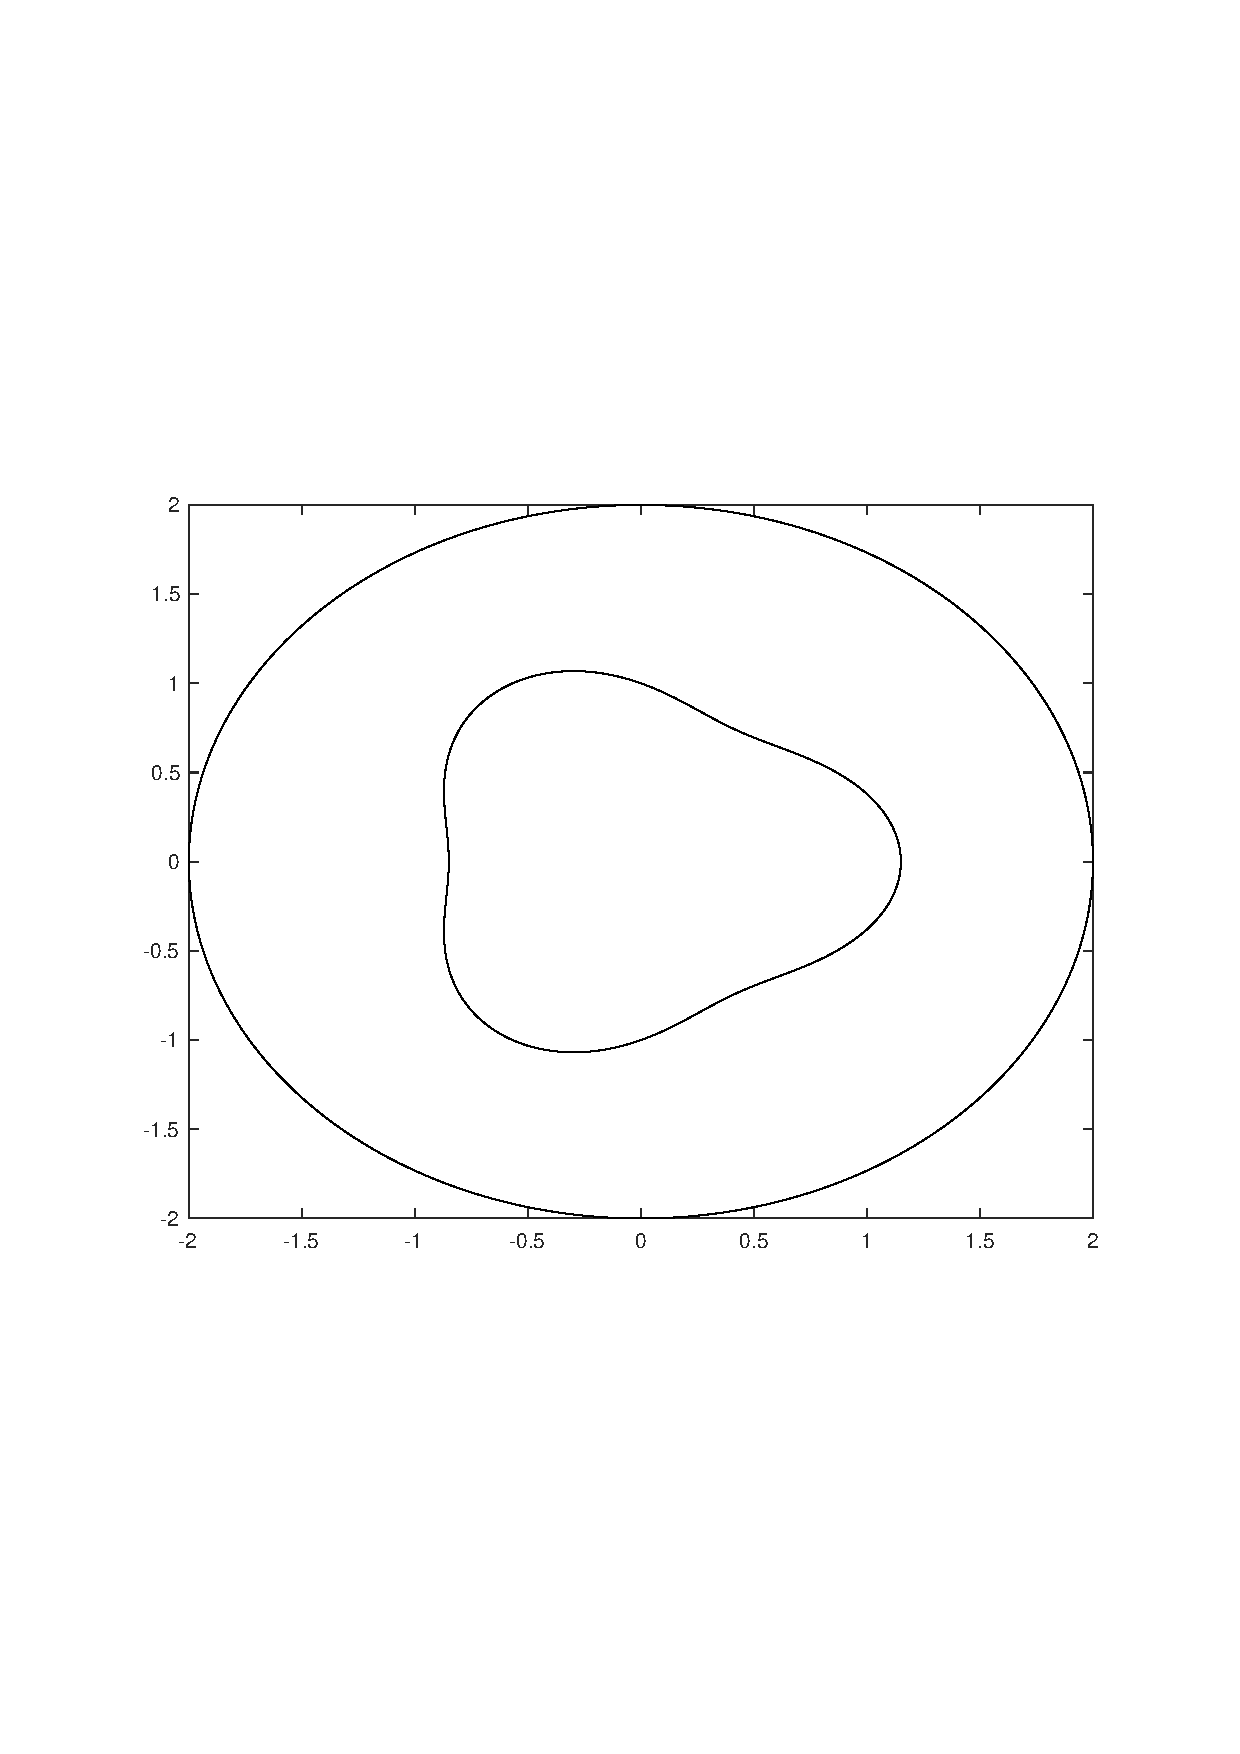
\includegraphics[scale=.5]{sample1.pdf}
	\vspace*{-3.5cm}
\end{figure}

 Параметричне задання області має вигляд
  \begin{equation*}
 \begin{split}
 	&\Gamma_1= \{x(s)=(r(s)\cos(s), r(s)\sin(s)),\ s\in[0,2\pi]\},\\
	&\Gamma_2= \{x(s)=(2\cos(s),2\sin(s)),\ s\in[0,2\pi]\},
 \end{split}
 \end{equation*}
 де $r(s)=1+0.15\cos(3s)$.
 
 Розв'язок шукатимемо в точці $x=(1, -1.5)\in \Omega$.
 
\begin{center}
\begin{tabular}{ |c|c|c| } 
\hline
      \multicolumn{3}{|l|}{\quad\quad\quad\quad\quad\quad\quad\quad\quad\quad\quad\quad\quad\quad $\tilde{u}(x)$} \tabularnewline
 \hline
 m & \shortstack{$A_0=A_1=A_2=1, \nu=0.5$}  & \shortstack{$A_0=0.1, A_1= 1,A_2=0, \nu=0.9$}  \\ 
 \hline
 4 & 2.1772 & 1.9093 \\ 
 8 & 2.2293 & 1.9261 \\ 
16 & 2.2374 & 1.9296 \\ 
32 & 2.2369 & 1.9295 \\ 
64 & 2.2369 & 1.9295 \\ 
128 & 2.2369 & 1.9295 \\
 \hline
\end{tabular}
 \captionof{table}{Наближення розв'язку при збільшенні $m$ і зміні основних параметрів}
 \end{center}

\subsection{Приклад 2}
Розглянемо крайову задачу з точним розв'язком
$$u(x)=G(x,y^*),$$
де $G(x,y^*)$ - звуження фундаментального розв'язку бігармонійного рівняння, $y^*\notin\Omega$.

Функції, що задані на $\Gamma_2$, мають вигляд

 \begin{gather*}
	g(x) = \frac{\partial G(x,y^*)}{\partial n},\\
	q(x) = M_xG(x,y^*).
 \end{gather*}


\subsubsection{Приклад 2.1}
\begin{figure}[h!]
\centering
	\vspace*{-4cm}
	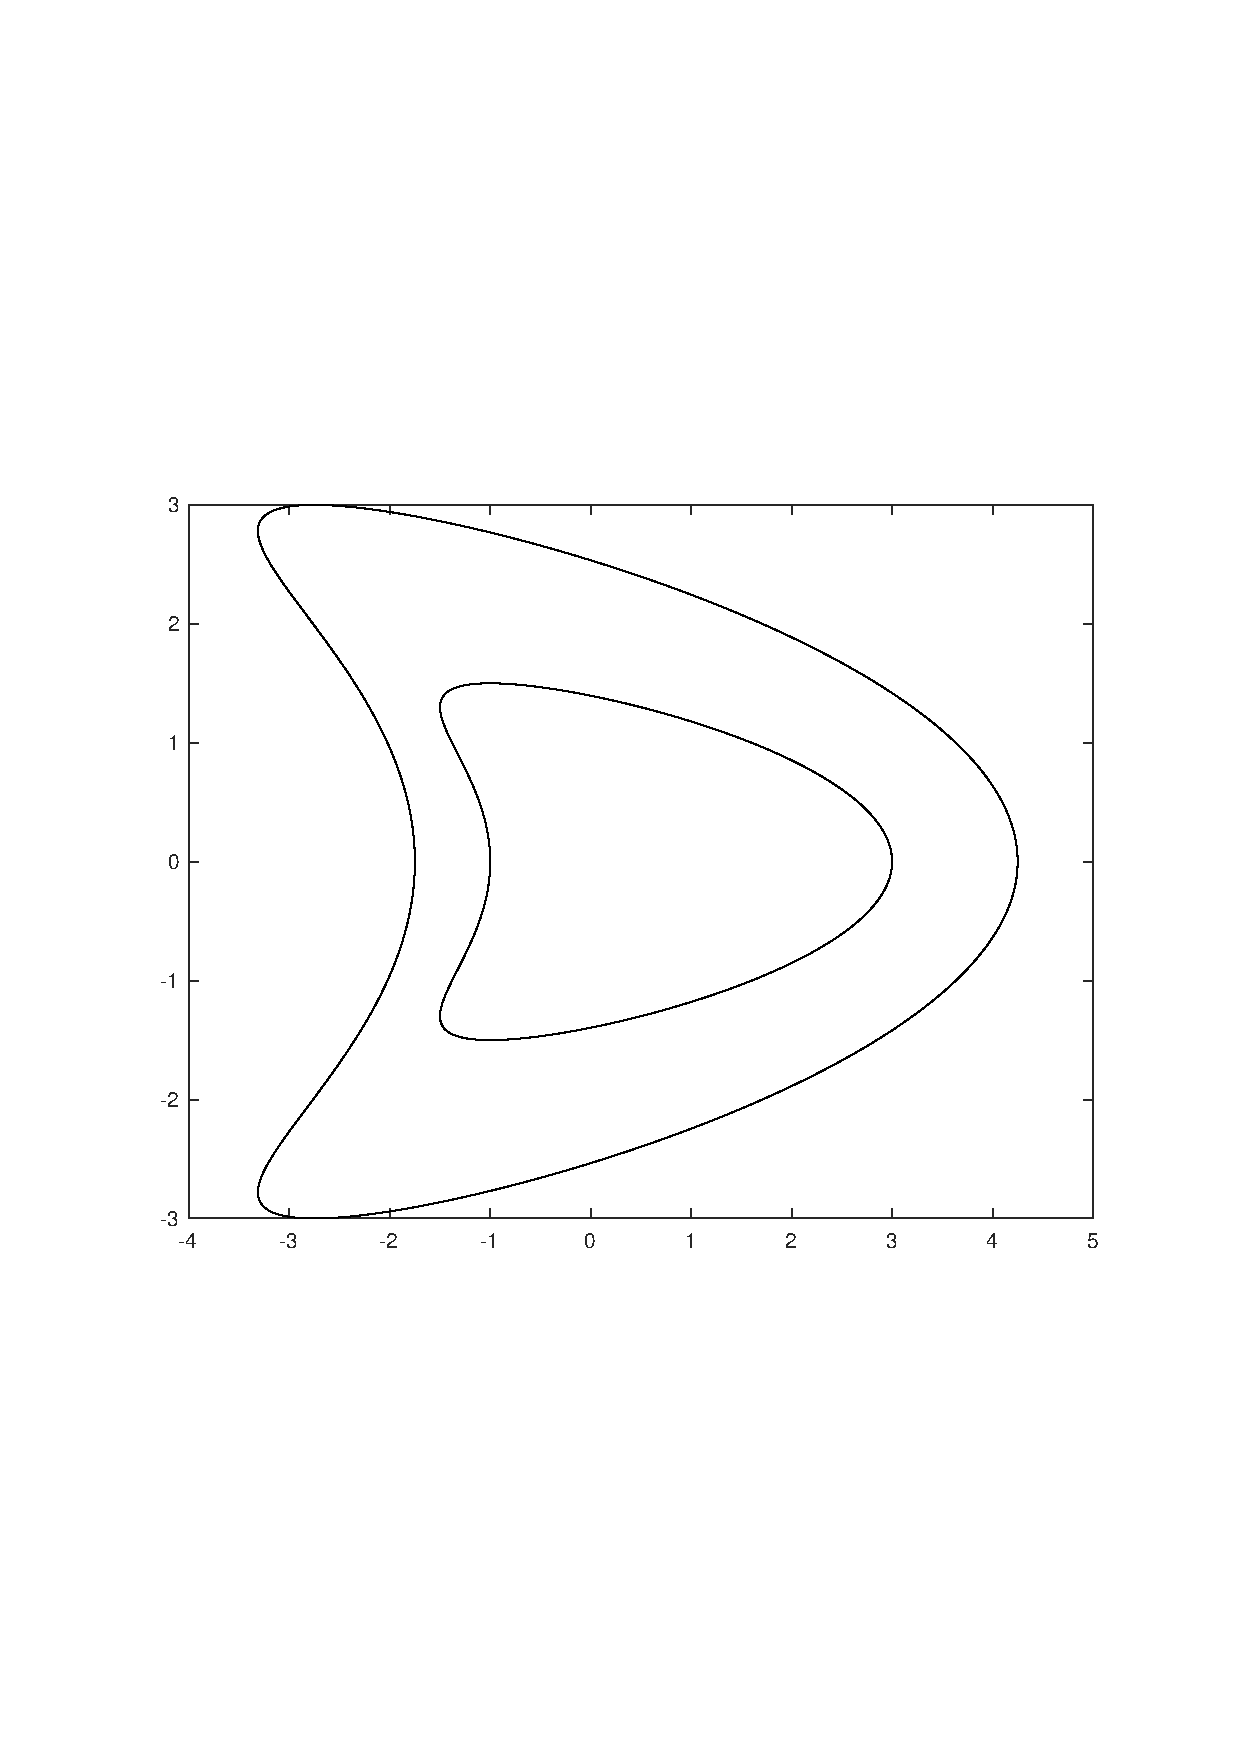
\includegraphics[scale=.5]{sample2.pdf}
	\vspace*{-4cm}
\end{figure}

 Параметричне задання області має вигляд
  \begin{equation*}
 \begin{split}
 	&\Gamma_1= \{x(s)=(3\cos(s) + 2\cos(2s) - 0.75, 3\sin(s)),\ s\in[0,2\pi]\},\\
	&\Gamma_2= \{x(s)=(2\cos(s)+\cos(2s),1.5\sin(s)),\ s\in[0,2\pi]\}.
 \end{split}
 \end{equation*}
 
 Розв'язок шукатимемо в точці $x=(0, -2)\in \Omega$.
 
\begin{center}
\begin{tabular}{ |c|c| } 
\hline
 & $|\tilde{u}-u_{ex}|$ \\
 \hline
 m & \shortstack{$A_0=A_1=A_2=1, \nu=0.5$}  \\
 \hline
 4 & 0.00100300  \\ 
 8 & 0.00001130  \\ 
16 & 7.0444e-08  \\ 
32 & 5.4863e-11 \\ 
64 & 6.5824e-15 \\ 
128 & 6.5824e-17 \\
 \hline
\end{tabular}
%\caption{Приклад 2} 
\end{center}

\subsubsection{Приклад 2.2}

  \begin{equation*}
 \begin{split}
 	&\Gamma_1= \{x(s)=(3\cos(s) + 2\cos(2s) - 0.75, 3\sin(s)),\ s\in[0,2\pi]\},\\
	&\Gamma_2= \{x(s)=(2\cos(s)+\cos(2s),1.5\sin(s)),\ s\in[0,2\pi]\}.
 \end{split}
 \end{equation*}
 
\begin{figure}[h!]
\centering
	\vspace*{-4cm}
	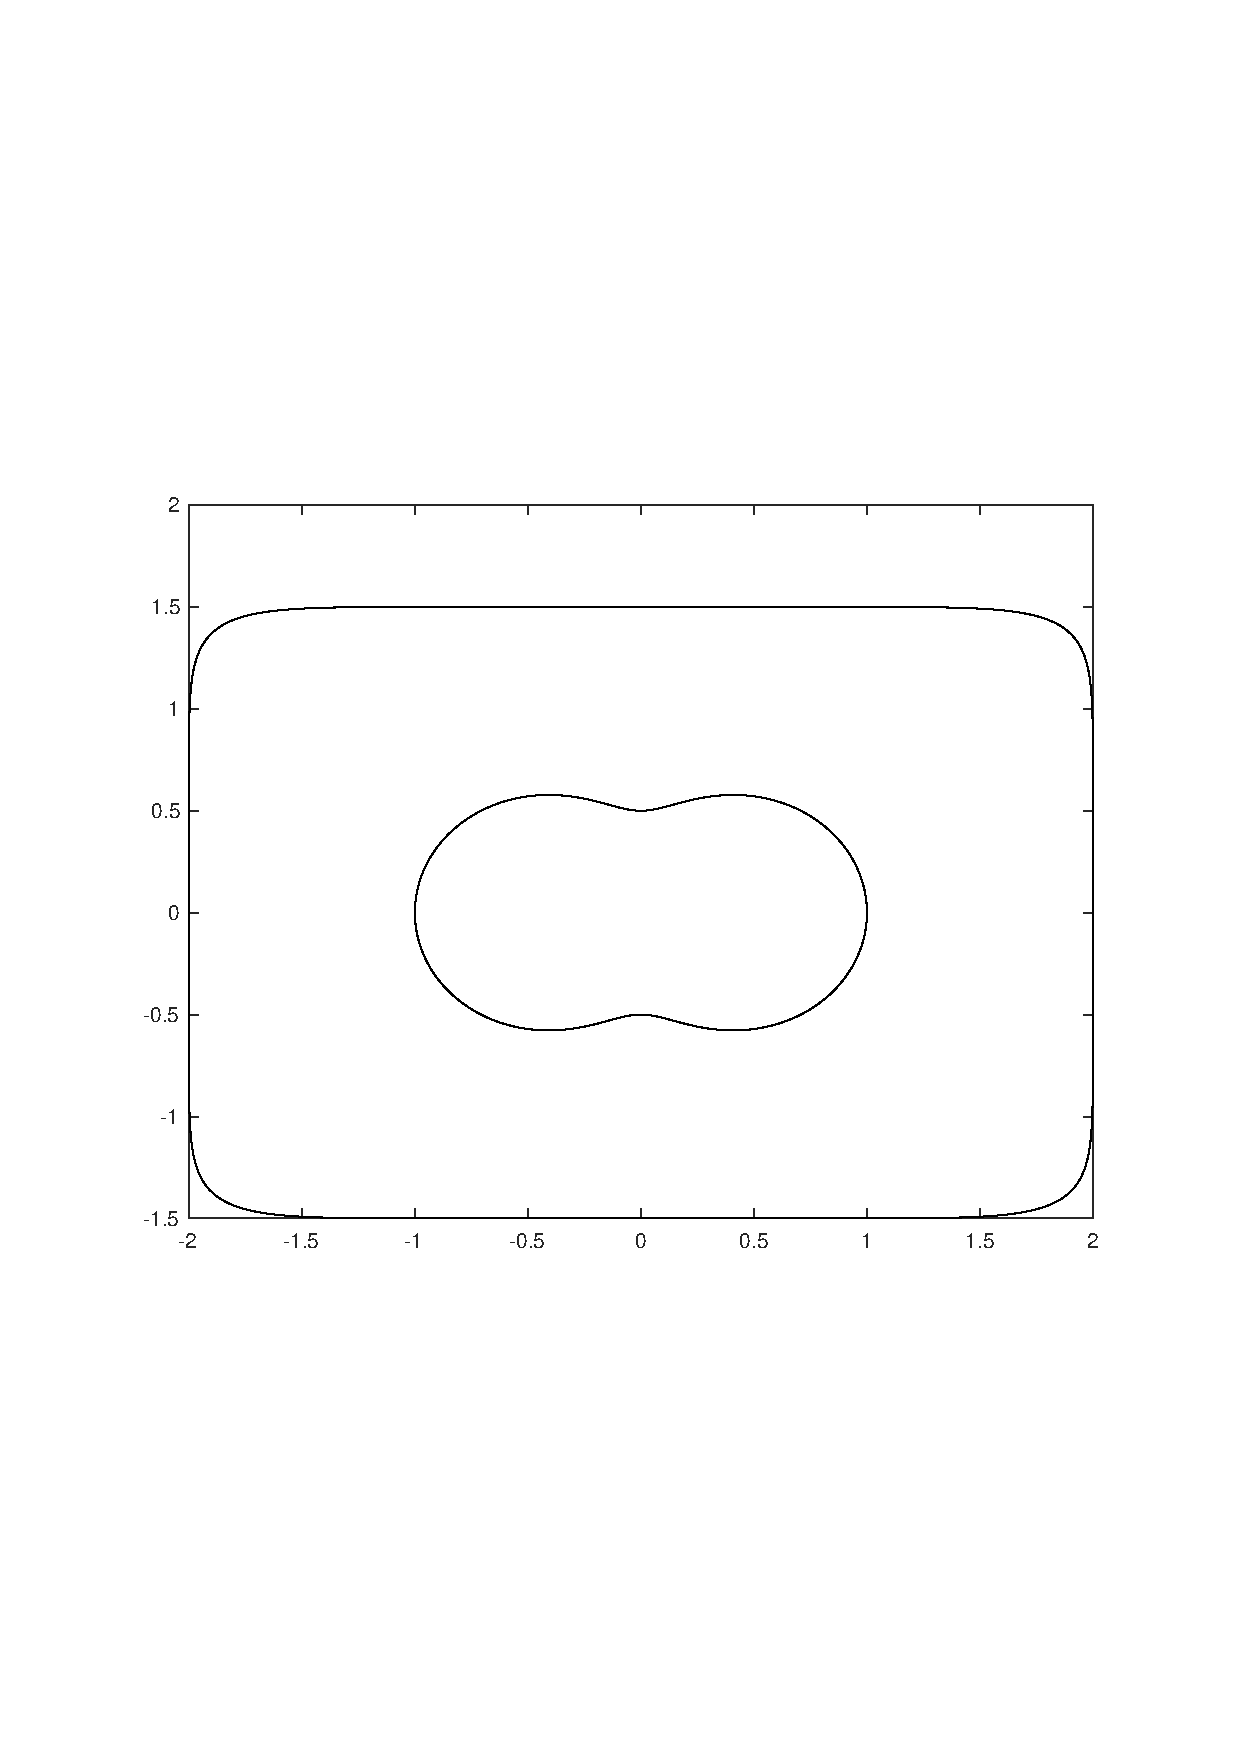
\includegraphics[scale=.5]{sample3.pdf}
	\vspace*{-4cm}
\end{figure}

 Розв'язок шукатимемо в точці $x=(0, -2)\in \Omega$.
 
\begin{center}
\begin{tabular}{ |c|c| } 
\hline
 & $|\tilde{u}-u_{ex}|$ \\
 \hline
 m & \shortstack{$A_0=A_1=A_2=1, \nu=0.5$}  \\
 \hline
 4 & 0.00100300  \\ 
 8 & 0.00001130  \\ 
16 & 7.0444e-08  \\ 
32 & 5.4863e-11 \\ 
64 & 6.5824e-15 \\ 
128 & 6.5824e-17 \\
 \hline
\end{tabular}
%\caption{Приклад 3} 
\end{center}

\chapter*{Висновки}
\addcontentsline{toc}{chapter}{Висновки}

\begin{thebibliography}{99}
 \addcontentsline{toc}{chapter}{Література}

\bibitem{chapko} 
Chapko R. Integral Equations for Biharmonic Data Completion / Roman Chapko, B. Tomas Johansson. - Inverse Problems and Imaging - 2019. - 16 p.
 
\bibitem{NonLinearIE} 
Chapko R. On The Non-Linear Integral Equation Method For The Reconstruction of The Inclusion in The Elastic Body / Roman Chapko, Vasyl Vavrychuk, Olha Ivanyshyn Yaman. - Lviv, 2019. - 17 p.
 
\bibitem{Uniqeness} 
Kress R. Inverse Dirichlet Problem and Conformal Mapping / Rainer Kress. - 2004. - 255-265 p.
 
\bibitem{Holmgren} 
Hedenmalm H. On the uniqueness theorem of Holmgren / Haakan Hedenmalm. - 2013. - 14 p.

\bibitem{ChapkoNonLinearIE} 
Chapko R. On a Hybrid Method For Shape Reconstruction of a Buried Object in an Elastostatic Half Plane / Roman Chapko. - Lviv, 2009. - 199-210 p.

\bibitem{KressNonLinearIE} 
Kress R. An Inverse Boundary Value Problem for the Oseen Equation / Rainer Kress, Sascha Meyer. - 18 p.
 
\bibitem{kress} 
Kress R. Linear Integral Equations / Rainer Kress. - New York : Springer, 1989. - 412 p.

\end{thebibliography}

\end{document}